%!TEX root = ../main.tex
%%%%%%%%%%%%%%%%%%%%%%%%%%%%%%%%%%
% Links:
%
% Difficulty:
% Companies: 
%%%%%%%%%%%%%%%%%%%%%%%%%%%%%%%%%%

\chapter{Trapping Water}
\label{ch:trapping_water}
\section*{Introduction}
Imagine being the only survivor of a plane crash in the middle of the pacific ocean and that you managed to get ashore to the Manra Island\footnote{Also called Sydney Island, is almost entirely of scrub forest, herbs, and grasses. The island is abandoned since 1963. 
%\vspace{-0.5cm}
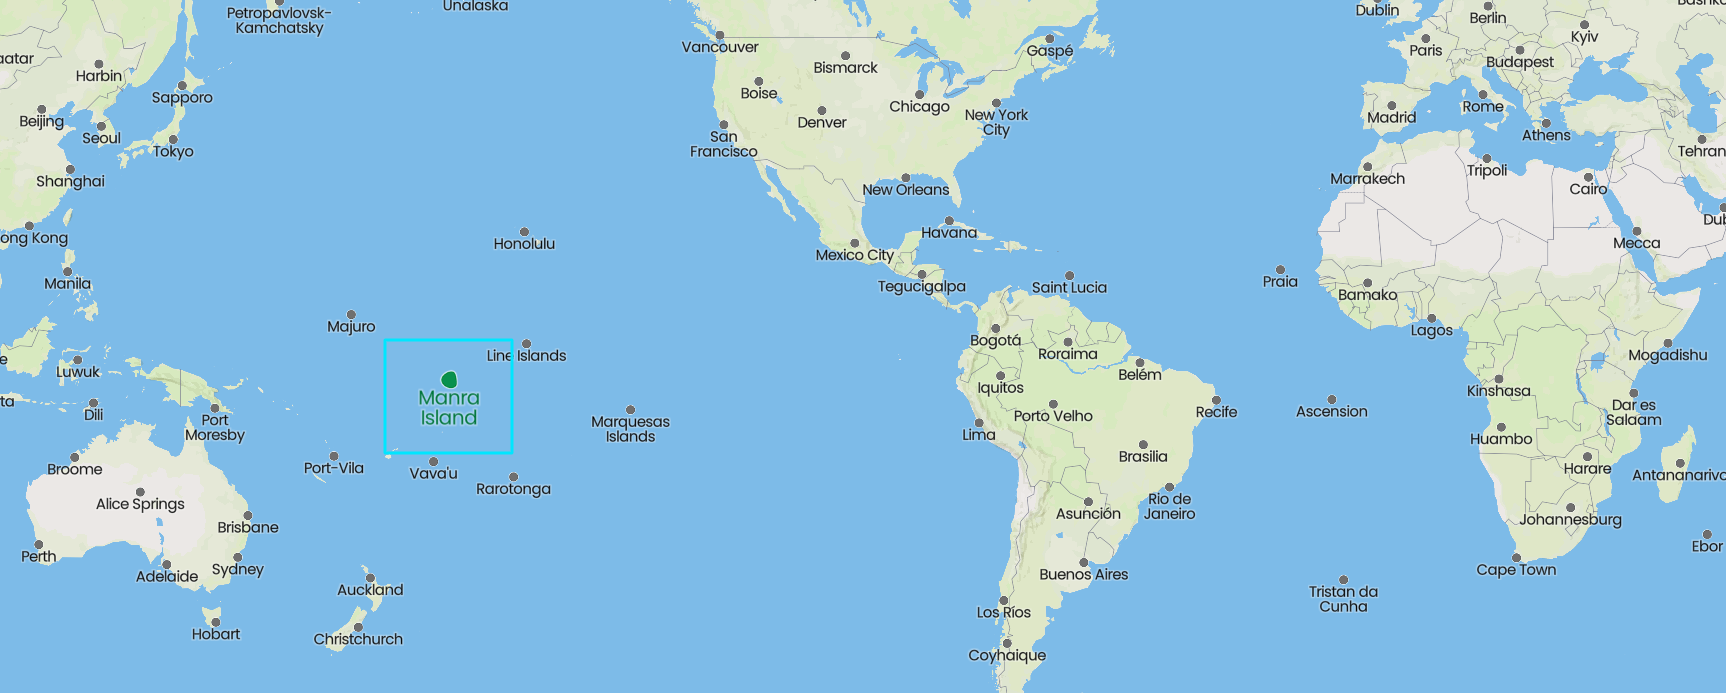
\includegraphics[]{sources/trapping_water/images/manra_island}} 
and that the only cargo item surviving the crash was a large number of plastic cubic boxes of size $1m^3$ and, two long, wide, and rigid sheets of acrylic glass \footnote{Poly (methyl methacrylate) (PMMA), is a transparent thermoplastic often used in sheet form as a lightweight or shatter-resistant alternative to glass.}.

Clearly one of your first worries would be to make sure you have enough water to be able to survive long enough for rescuers to find and save you.
You come up with the brilliant idea of arranging the boxes into piles of different heights each placed along the same direction  
at a certain distance from each other so that they form concave structures that sealed with the help of the plastic sheets collect rainwater as depicted in Figure \ref{fig:trapping_water_example1}. 

In order to figure out the best ways of arranging boxes so that the structure collects as much water as possible to take advantage of the scarce rain, you would like to calculate the total amount of water each possible boxes arrangement can hold.
In this chapter's problem we will investigate how this calculation can be carried out efficiently and, as we shall see, we will learn that there are a number of valid approaches that can be used.
We believe it is important to master the core concepts of all of them as their applicability extends further to the limited context of this specific problem and that, we can extract valuable lessons from each of them.
Moreover, this problems has been (and according to what interviewees across the globe still reports) a major hit in top tech companies, where it is still nowadays frequently asked during interviews.


\section{Problem statement}
\begin{exercise}
Write a function that takes as input an array of length $n$ of non-negative integers representing an elevation map (the height of each pile of boxes) where the width of each bar is $1$. 
The function should return the maximum amount of water that can be potentially trapped in between all the piles. 

	\begin{example}
		\label{ex:trapping_water:exmaple1}
		\hfill \\
		Given the array $H=[0,1,0,2,1,0,1,3,2,1,2,1]$ (see Figure \ref{fig:trapping_water_example1}), the function return $8$
	\end{example}

	\begin{example}
		\label{ex:trapping_water:exmaple2}
		\hfill \\
		Given the array $H=[3,2,0,0,4,4,1,2,5,4,0,2,1]$ (see Figure \ref{fig:trapping_water_example2}), the function return $14$
	\end{example}

\end{exercise}

\begin{figure}
	\centering
	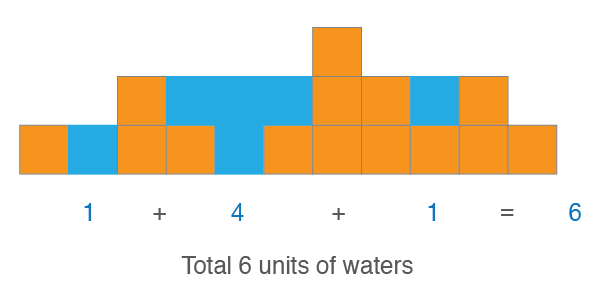
\includegraphics[scale=1.0]{sources/trapping_water/images/example1}
	\caption{Visual representation of the heightmap $H=[0,1,0,2,1,0,1,3,2,1,2,1]$ in the Example \ref{ex:trapping_water:exmaple1}. Blue squares represent water, while the red ones, boxes.}
	\label{fig:trapping_water_example1}
\end{figure}



\begin{figure}
	\centering
	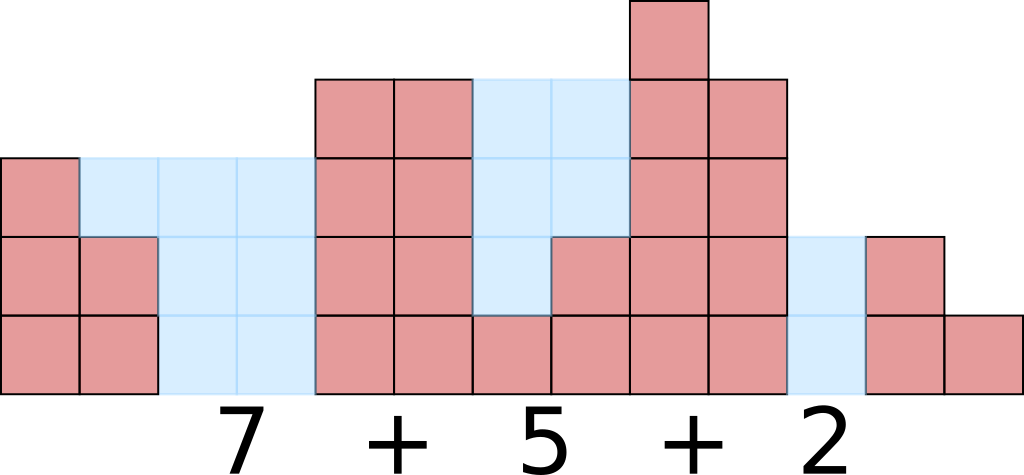
\includegraphics[scale=1.0]{sources/trapping_water/images/example2}
	\caption{Visual representation of the heightmap $H=[3,2,0,0,4,4,1,2,5,4,0,2,1]$ in the Example \ref{ex:trapping_water:exmaple2}. Blue squares represent water, while the red ones, boxes.}
	\label{fig:trapping_water_example2}
\end{figure}

%\section{Clarification Questions}
%
%\begin{QandA}
%	\item 
%	\begin{answered}
%		\textit{}
%	\end{answered}
%	
%\end{QandA}

\section{Discussion}
\label{trapping_water:sec:discussion}
There are at least three tecniques we can use to  solve this challenge so that that will satisfy the interviewer:
\begin{enumerate}
	\item Dynamic programming (Section \ref{trapping_water:sec:dp})
	\item Two pointers (Section \ref{trapping_water:sec:two_pointers})
	\item Stack (Section \ref{trapping_water:sec:stack})
\end{enumerate}
But as usual, we will start our discussion on the problem's solutions by looking at a possible brute-force solution before  passing onto more sophisticated and faster solutions.

\subsection{Brute-force}
\label{trapping_water:sec:bruteforce}

A possible way to brute-force  solve this problem comes from the fact that each element of the array (pile) can potentially hold some water provided that there are other two bars surrounding it (one at its left and one at its right), with height equal or higher.
If that is the case then, we can safely add enough water so its level reaches an height equal to the smallest of the two surrounding piles.
For instance w.r.t. to \ref{ex:trapping_water:exmaple2}, we can see that for the element at index $6$ (having height $1$), the highest bars on its left and right have height $3$ and $4$, respectively. 
We can add water on top of the pile at index $6$ up to a height of $3$ (the minimum between $3$ and $4$) without risking the water spilling out.
Figure \ref{fig:trapping_water_example3} depicts how the pile marked with the question mark can be processed using this approach i.e. by calculating the minimum between $b_l$ and $b_r$ (the height of the highest bars on its left and right, respectively).

If on the other hand, a pile is higher than both the highest bars on its left and right side, then it is impossible to add any water on it (this is the case always the case when processing the highest bar on the histogram).


\begin{figure}
	\centering
	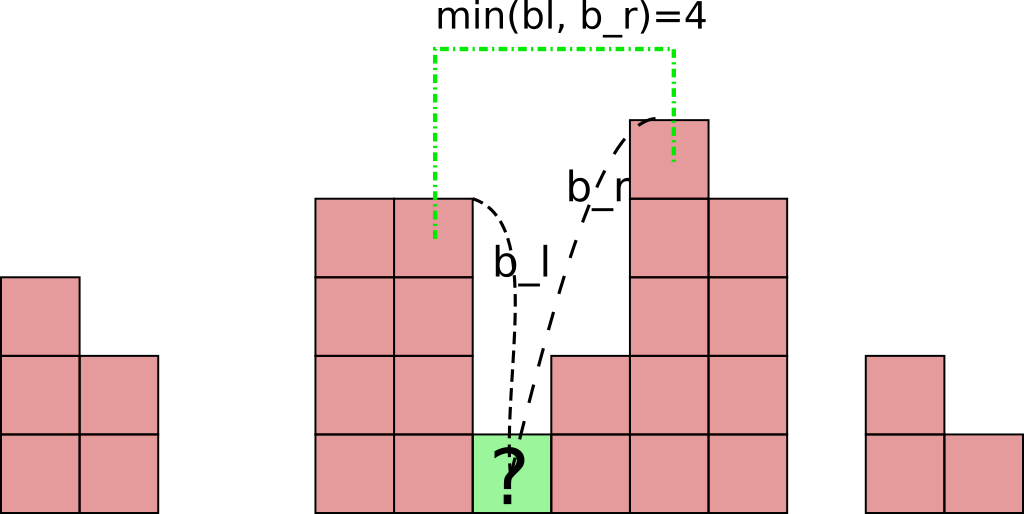
\includegraphics[scale=1.0]{sources/trapping_water/images/example3}
	\caption{Calculation of the water we can fit on top of a pile using the information about the highest bars surrounding it.}
	\label{fig:trapping_water_example3}
\end{figure}

To summarize, we can find the answer to an instance of this problem by calculating the amount of water we can place on top of each pile \inline{H[i]} by:
\begin{enumerate}
	\item find the height of the highest bars on the left (\inline{b_l}) and right (\inline{b_r}) of \inline{H[i]};
	\item add \inline{std::max(0, std::min(b_l, b_r) - H[i])} to the final answer. 
\end{enumerate}
\inline{b_l} and  \inline{b_r} can be implemented with a simple linear search which is performed for all the elements of $H$ causes the complexity of the full algorithm to reach $O(n^2)$.
Moreover, we should notice that the first and the last element will never be able to hold any water as those elements have no bars on their left and right, respectively (any water placed on top of them will inevitably spill outside the structure).

Listing \ref{list:trapping_water:bruteforce} shows a possible implementation of this idea. 
Notice how the \inline{std::max_element} function from C++ STL can be employed elegantly to calculate $b_l$ and $b_r$.

\lstinputlisting[language=c++, caption=Brute-force solution.,label=list:trapping_water:bruteforce]{sources/trapping_water/trapping_water_solution1.cpp}


\subsection{Dynamic Programming}
\label{trapping_water:sec:dp}
The solution proposed in Section \ref{trapping_water:sec:bruteforce} is far from optimal, but it can be transformed into a pretty good one if we can somehow precalculate the values of $b_l$ and $b_r$ in linear time,
We have discussed in great detail how this can be achieved in Chapter \ref{ch:greatest_right}, and it can indeed be accomplished in linear time. 

Therefore all it is necessary is to use pre-calculate (reusing the logic in Listing \ref{list:greatest_right_final1} for instance) $R$, and $L$ each of length $n$ (same as $|H|$) where: 
\begin{itemize}
	\item $R[i]$ contains the value of the highest bar among all elements of the input with index $j > i$ (on the right of, and not considering, $i$).
	\item symmetrically, $L[i]$ contains the value of the highest bar among all elements of the input with index $j < i$ (on the left of, and not considering, $i$).
\end{itemize}

Armed with these two arrays, the same algorithm used in Section \ref{trapping_water:sec:bruteforce} can be turned into an elegant and efficient solution that will make any interviewer smile as shown in 
Listing \ref{list:trapping_water:dp}.

\lstinputlisting[language=c++, caption={Dynamic programming, $O(n)$ time and space solution.},label=list:trapping_water:dp]{sources/trapping_water/trapping_water_solution2.cpp}

The code is clearly divided into two separate and kind of independent steps each of time complexity $O(n)$. 
\begin{enumerate}
	\item vectors \inline{R} and \inline{L} are filled up by using the function \inline{max_left_it}. It is worth noticing here how we are able to calculate $R$ only using the function \inline{max_left_it} (that as hinted by its name calculates the maximum value to the left of each element of the input array), by providing the input to \inline{max_left_it} reversed reversing what comes out of it; Figures \ref{fig:trapping_water_DPL} and \ref{fig:trapping_water_DPR} show a representation of $L$ and $R$. If we superimpose them we can visualize the amount of water we can trap between the piles as shown in  Figure 
	\ref{fig:trapping_water_DPRL}.
	\item the answer calculated by summing up the amount of water that can stand on top of a pile by using the values of  \inline{R[i]}, \inline{L[i]} and \inline{height[i]} as also discussed in Section \ref{trapping_water:sec:discussion}.
\end{enumerate}

Listing \ref{list:trapping_water:dp} has a time complexity of $O(n)$ because the computation of $L$ and $R$ can be done in linear time, while calculating the final answer can be done in a single pass over the array. The space complexity is linear as well because the arrays $L$ and $R$ have both size proportional to $n$.

\begin{figure}
\centering
\begin{subfigure}[b]{0.95\textwidth}
   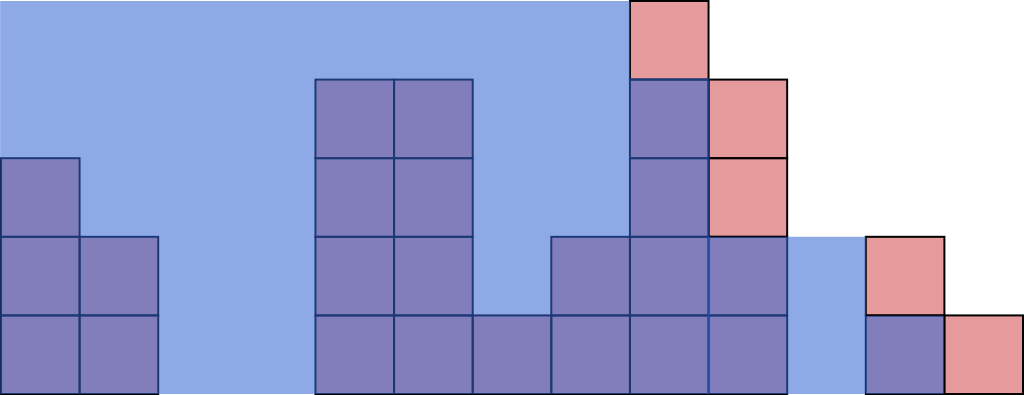
\includegraphics[width=1\linewidth]{sources/trapping_water/images/DPR}
   \caption{Representation of the highest value to the right of a pile. The level of color \textcolor[HTML]{3268d5}{$\blacksquare$} on top of each pile marks the maximum height of another pile to its \textbf{right}.}
   \label{fig:trapping_water_DPL}
\end{subfigure}

\begin{subfigure}[b]{0.95\textwidth}
   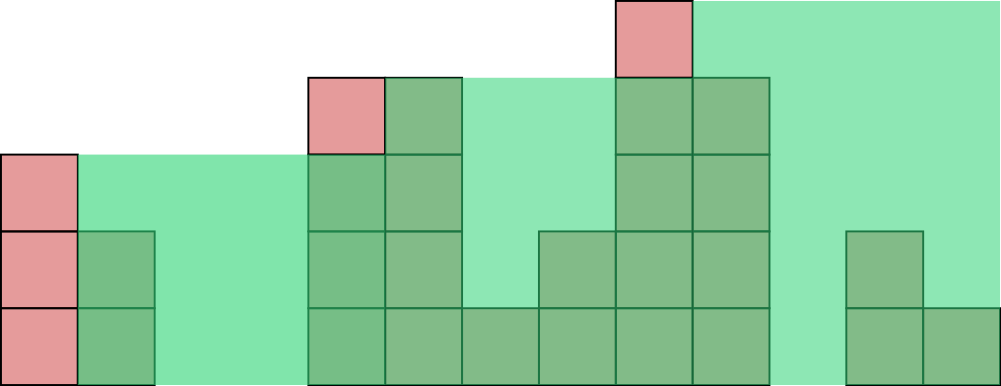
\includegraphics[width=1\linewidth]{sources/trapping_water/images/DPL}
   \caption{Representation of the highest value to the left of a pile. The level of color \textcolor[HTML]{32d579}{$\blacksquare$} on top of each pile marks the maximum height of another pile to its \textbf{left}.}
   \label{fig:trapping_water_DPR}
\end{subfigure}

\begin{subfigure}[b]{0.95\textwidth}
   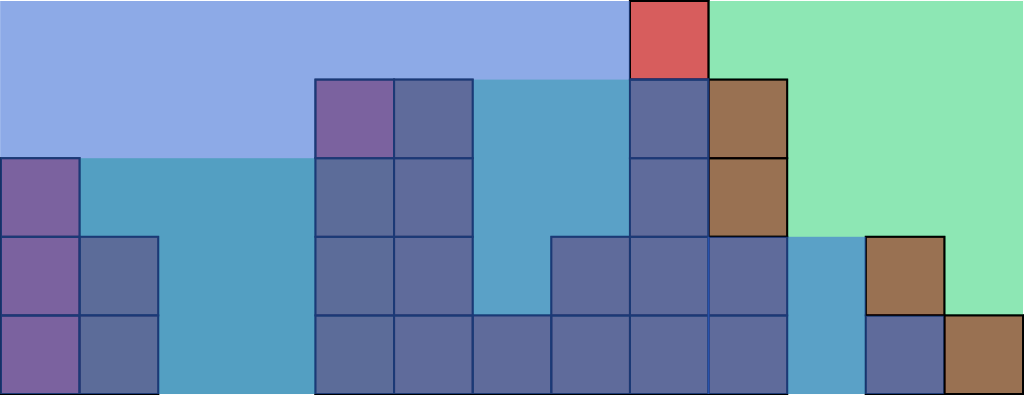
\includegraphics[width=1\linewidth]{sources/trapping_water/images/DPLR}
   \caption{Superimposition of Figures \ref{fig:trapping_water_DPL} and \ref{fig:trapping_water_DPR}. Cells colored in \textcolor[HTML]{5aa1c7}{$\blacksquare$} represent the intersection between cells colored in \textcolor[HTML]{3268d5}{$\blacksquare$} in Figure \ref{fig:trapping_water_DPL} and cells colored in \textcolor[HTML]{32d579}{$\blacksquare$} in Figure \ref{fig:trapping_water_DPR}. Those are the cells that can trap water.}
   \label{fig:trapping_water_DPRL}
\end{subfigure}
\caption{}
\label{fig:trapping_water:dprl_main}
\end{figure}



\subsection{Two pointers solution}
\label{trapping_water:sec:two_pointers}
Despite the fact that the solution presented in Section \ref{trapping_water:sec:dp} is already a good time-complexity-wise, we can definitely do better and lower the space complexity down to $O(1)$.
The key idea is that, we do not really need to store the information of $L$ and $R$ in their entirety.
Whenever we are calculation the contribution of a pile,  we only need a single value from both $L$ and $R$; nothing else.
Once we are done with that pile we can freely discard the corresponding elements in $L$ and $R$ we have used because they are of never to be used in the future as they do not play any role in the calculation of the contribution to the final answer of any other element of the input array $H$.
The solution proposed in this Section uses a two-pointers technique which maintain two \textit{rolling} maximum values, $m_l$ and $m_r$, one for the left and one for the right of a single pile.
When processing the pile at index $i$, $m_l$ and $m_r$ contain the maximum value to the its left and right, respectively (the same information stored in $L[i]$ and $R[i]$).

The input arrays is traversed from left to right using two pointers $l$ and $r$, which are initialized to the beginning and the end of the input array, respectively.
$m_l$ and $m_r$ are initialized to $0$.
The idea is that we process one of the elements pointed by $l$ or $r$ depending on which is larger. 
$m_l$ and $m_r$ always contain the largest element to the left of $l$ and, simmetrically $m_r$ contains the largest element to the right of $r$. 

We process the smallest element between $H[l]$ and $H[r]$ and in particular if \inline{H[l] <= H[r]} is:
\begin{description}
	\item[true:]  then the contribution of \inline{H[l]} is bounded by \inline{m_l} (because \inline{H[r] >= H[l]}. $l$ is moved towards the center (we have considered the contribution of this cell and we can move forward).\\
	\item[false:] then the contribution of \inline{H[j]} is bounded by \inline{m_r} (because \inline{H[l] >= H[r]}. $r$ is moved towards the center (we have considered the contribution of this cell and we can move forward). \\
\end{description}

An implementation of the idea above is shown in Listing \ref{list:trapping_water:two_pointers}.

\lstinputlisting[language=c++, caption={Two pointers solution, $O(n)$ time and  $O(1)$ space, solution to the problem of calculating the amount of water trapped between buildings.},label=list:trapping_water:two_pointers]{sources/trapping_water/trapping_water_solution3.cpp}

The code is pretty self explanatory but it is worth noticing that all the elements of the input array will be  considered eventually because either $l$ or $r$ are moved one one step closer to each other at each iteration. 

This approach has a time complexity of $O(n)$ (we cannot do better than this because at least we have to touch all the elements of the input at least once) and a space complexity of $O(1)$ which is optimal.

We believe this is the solution the interviewer is hoping to see. 


% review done 13/07

\subsection{Stack based solution}
\label{trapping_water:sec:stack}
There is another way of solving this problem in linear time that makes good use of a stack. The main idea is to loop through $H$ one element $p_i$ (pile at index $i$ in $H$) at the time and try to place $p_i$ on the stack in such a way that the values in the stack are always in a decreasing order (from top to bottom).
We start with an empty stack $S$ and for each pile $p_i \in H$ we do one of the two following operations depending on whether $p_i$  is lower than the current top of the stack $s_{top}$:
\begin{description}
	\item[$p_i < s_{top}$] the current top of the stack is higher than $p_i$ which means that $s_{top}$ bounds $p_i$ from the left. In this case we simply add it to the top of the stack. At this point the stack is still ordered in a decreasing fashion.
	\item[$p_i \geq s_{top}$] we have a pile that is higher or equal to the $s_{top}$. Therefore if we want to place $p_i$ on the stack and maintain the ordering, we need to remove as many elements as necessary until we are left with a top of the stack that is higher of $p_i$, or the stack is fully empty (this happens for instance, but not only, when $p_i$ is the highest pile in $H$).
	However each each pile that is removed together with $p_i$  form a rectangular area that can trap some water. Why is that? Well, the removed pile is bounded from the left by some other pile (this is guaranteed by how elements are inserted in the stack, or more simply by the ordering the stack maintains) and to the right by $p_i$ itself. 
	How much water exactly? 
	The contribution of the removed element $S_{oldtop}$ is calculated as the area of a rectangle of base equal to the distance between the two bounding bars ($p_i$ and the element before $S_{oldtop}$) and and height that is equal to the minimum of the heights between the two bounding bars \textbf{minus} $S_{oldtop}$. Clearly if there is no bar left in the stack once we remove $S_{oldtop}$, there is no way we can trap water and therefore we add nothing to the final answer. 
\end{description}
Figure \ref{fig:trapping_water:stack_ex} shows a step-by-step  execution of this algorithm.

A possible implementation of this idea is shown in Listing \ref{list:trapping_water:stack}.
Notice that the real work happens inside the \inline{while} loop and that the pile we calculate the contribution is named \inline{old_top} while the bar on the left and right are named \inline{bar_left} and \inline{bar_right} (equivalent to $p_i$) respectively. 
Moreover, no matter the stack is unwound or not, \inline{bar_right} is \textbf{added} to the stack because when controls reaches line $21$ it will be either the only bar in the stack of it will be smaller than the current top (order is restored).



The complexity of this approach is linear in both time and space .

\lstinputlisting[language=c++, caption={Stack based solution, $O(n)$ time and  space solution.},label=list:trapping_water:stack]{sources/trapping_water/trapping_water_solution4.cpp}

 


\begin{figure}
	\vspace{-0.4in}
	%\hspace*{-0.3in}
	\centering
	\begin{subfigure}[t]{0.24\textwidth}
		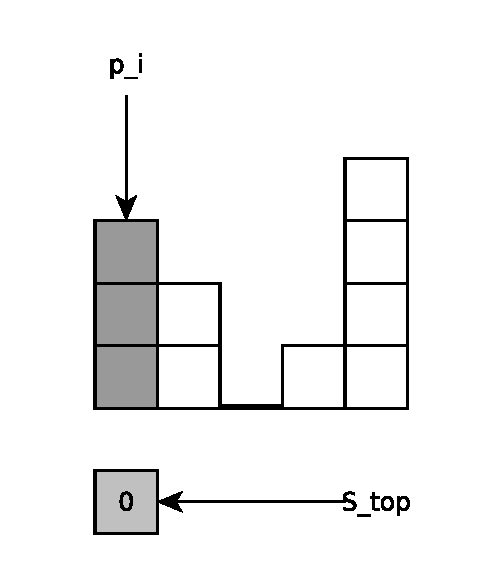
\includegraphics[width=1\linewidth]{sources/trapping_water/images/stack_ex1}
		\caption{At the beginning the stack is empty and pile $0$ is pushed onto it.}
		\label{fig:trapping_water:stack_ex1}
	 \end{subfigure}
	\hfill
	\begin{subfigure}[t]{0.24\textwidth}
		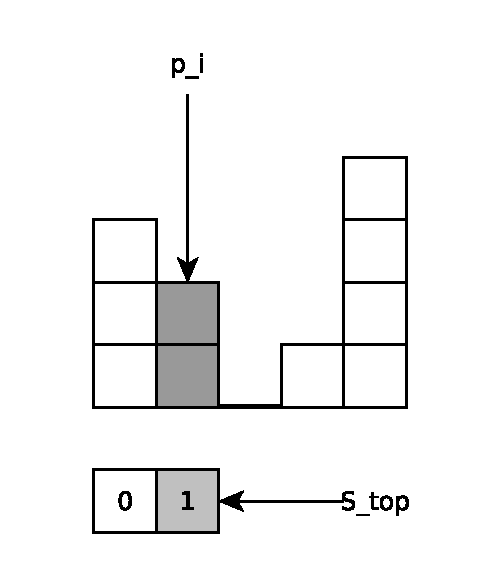
\includegraphics[width=1\linewidth]{sources/trapping_water/images/stack_ex2}
		\caption{Pile  at index $1$ is 2 boxes tall and it is smaller than the current top of the stack having height equal to $3$. Pile $1$ is pushed onto the stack.}
		\label{fig:trapping_water:stack_ex2}
	 \end{subfigure}
	 \hfill
	 \begin{subfigure}[t]{0.24\textwidth}
		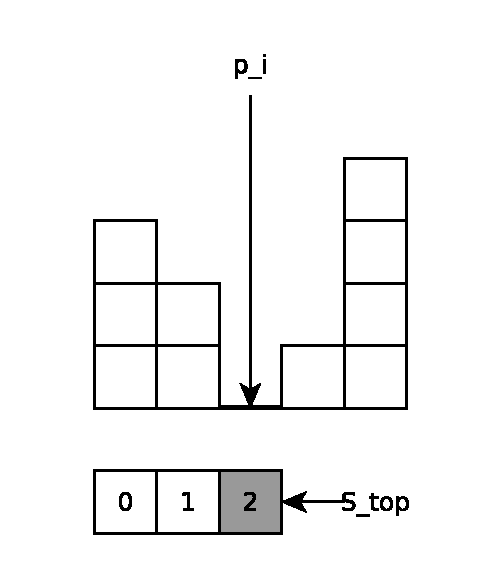
\includegraphics[width=1\linewidth]{sources/trapping_water/images/stack_ex3}
		\caption{Pile $2$ has height $0$ which is smaller than the top of the stack and it is thus pushed on top.}
		\label{fig:trapping_water:stack_ex3}
	 \end{subfigure}
	 \hfill
	 \begin{subfigure}[t]{0.24\textwidth}
		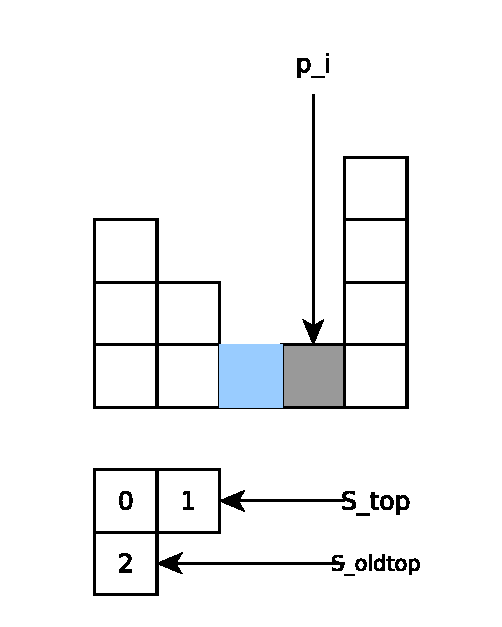
\includegraphics[width=1\linewidth]{sources/trapping_water/images/stack_ex4}
		\caption{Pile $3$ has height $1$ which is higher than the current top of the stack. We therefore pop the current top (we store it in $S_{oldtop}$) and we calculate its contribution to the final answer by using it, the new top and $p_i$. The area that can be filled with water is highlighed in light blue \textcolor[HTML]{99ccff}{$\blacksquare$}. At this point the new top is higher than $p_i$ and we can push it onto the stack which now contains $\{0,1,3\}$.}
		\label{fig:trapping_water:stack_ex3}
	 \end{subfigure}
	 \hspace*{-0.5in}
	 \begin{subfigure}[t]{0.24\textwidth}
		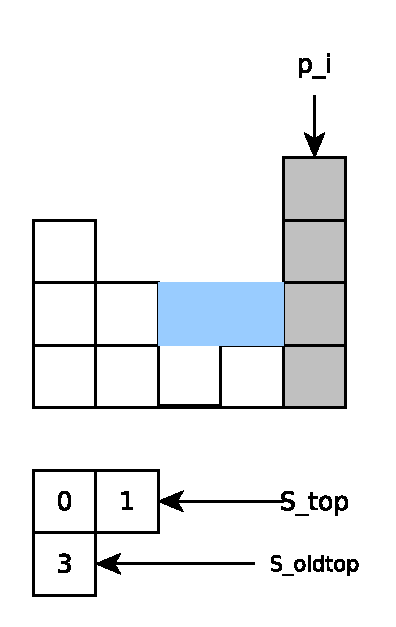
\includegraphics[width=1\linewidth]{sources/trapping_water/images/stack_ex5}
		\caption{The last pile is the highest of all and therefore it is also taller than the top of the stack. We pop the current top pile $3$ of height $1$ and we calculate its contribution to the final answer; an area of two squares in this case (highlighed in light blue \textcolor[HTML]{99ccff}{$\blacksquare$}).}
		\label{fig:trapping_water:stack_ex3}
	 \end{subfigure}
	 \hfill
	 \begin{subfigure}[t]{0.24\textwidth}
		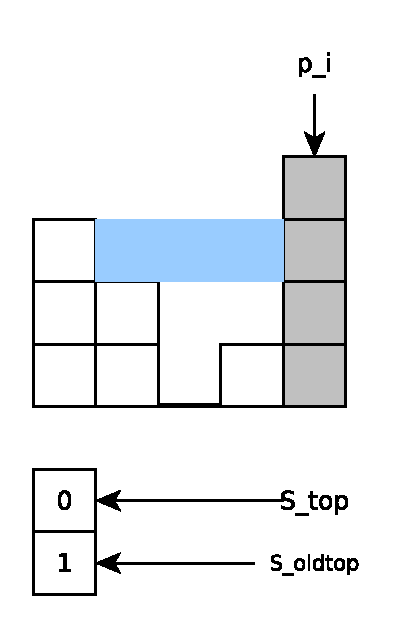
\includegraphics[width=1\linewidth]{sources/trapping_water/images/stack_ex6}
		\caption{At this point we are still trying to insert pile $4$ onto the stack, but its height is still higher than the current top of the pile (pile $1$ of height $2$). Therefore, we pop the current top and calculate its contribution to the final answer (the three cells highlighed in lighe blue \textcolor[HTML]{99ccff}{$\blacksquare$}).}
		\label{fig:trapping_water:stack_ex3}
	 \end{subfigure}
	 \hfill
	 \begin{subfigure}[t]{0.24\textwidth}
		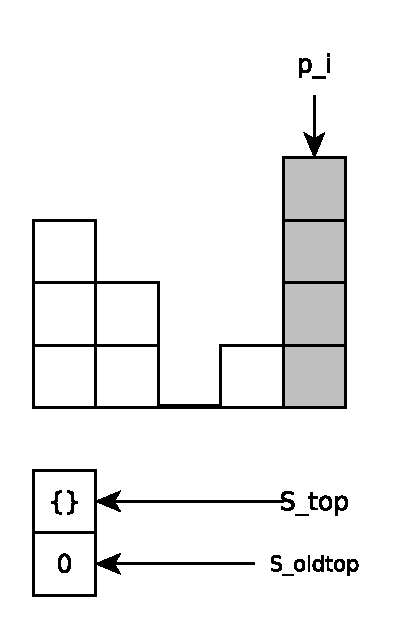
\includegraphics[width=1\linewidth]{sources/trapping_water/images/stack_ex7}
		\caption{At this point there is only one element in the stack (pile $0$) which happens to be smaller then $p_i$. We therefore move the current top to $S_{oldtop}$ and we would normally calculate its contribution to the final answer, but at this point the stack is empty which means pile $0$ is not bound by any other pile to the left. $p_i=4$ is finally added to the stack.}
		\label{fig:trapping_water:stack_ex3}
	 \end{subfigure}
	 \hfill
	 \begin{subfigure}[t]{0.24\textwidth}
		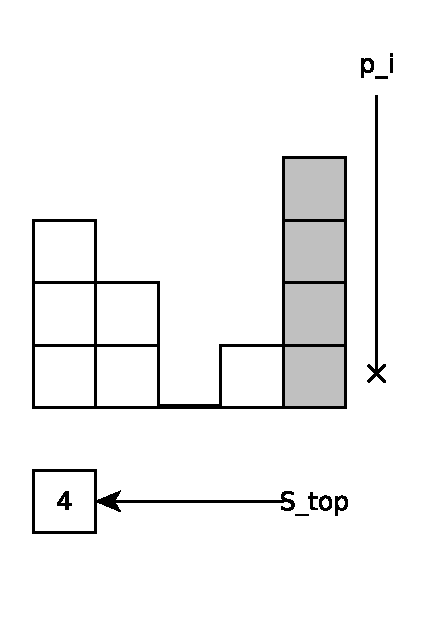
\includegraphics[width=1\linewidth]{sources/trapping_water/images/stack_ex8}
		\caption{At this point the algorithm terminates as there is no more pile to process.}
		\label{fig:trapping_water:stack_ex3}
	 \end{subfigure}
	 \caption[Execution of the stack based algorithm.]{Execution of the algorithm discussed in Section \ref{trapping_water:sec:stack} and implemented in Listing \ref{list:trapping_water:stack} on the input $H=\{3,2,0,1,4\}$. The final answer is the sum of the light blue cells \textcolor[HTML]{99ccff}{$\blacksquare$}, for a total of $6$ squares worth of water that can be trapped by this particular pattern of piles.}
	 \label{fig:trapping_water:stack_ex}
\end{figure}